\documentclass[aspectratio=169, 11pt]{beamer}

% --- Packages & Setup ---
\usepackage[utf8]{inputenc}
\usepackage[T1]{fontenc}
\usepackage{xcolor}
\usepackage{booktabs}
\usepackage{graphicx}
\usepackage{tikz}
\usetikzlibrary{calc}

% Try loading Open Sans; fallback if missing
\IfFileExists{opensans.sty}{\usepackage[default,scale=0.95]{opensans}}{}

% --- Branding Colors ---
\definecolor{amritaMaroon}{HTML}{A4123F}

% --- Theme Setup ---
\usetheme{Madrid}
\usecolortheme[named=amritaMaroon]{structure}
\setbeamertemplate{navigation symbols}{}
\setbeamertemplate{footline}[frame number]

\begin{document}

% --- CUSTOM TITLE SLIDE ---
\begin{frame}
    % Corner Box Indicator
    \begin{tikzpicture}[remember picture,overlay]
        \node[fill=amritaMaroon, text=white, font=\bfseries\footnotesize, anchor=north east, rounded corners=2pt, inner sep=5pt]
        at ($(current page.north east) + (-0.2cm,-0.2cm)$)
        {Type 1: Research Project};
    \end{tikzpicture}

    \centering
    % Adjusted logo size to save vertical space
    
\includegraphics[width=2.2cm]{logo_square.png}
    \vspace{0.2cm}

    {\Large \textbf{\textcolor{amritaMaroon}{Explainable Federated Analytics for Multivariate Time-Series Forecasting with Personalized Drift Adaptation}}} \\
    \vspace{0.1cm}
    {\small \textbf{Team Number: 28}} \\
    \vspace{0.1cm}

    % Student Table - Adjusted size to fit 5 students
    \begin{table}
        \centering
        \footnotesize % Reduced font size slightly
        \renewcommand{\arraystretch}{1.0} % Tightened row spacing
        \begin{tabular}{|c|c|l|}
            \hline
            \textbf{S.No} & \textbf{Register Number} & \textbf{Student Name} \\
            \hline
            1 & CB.SC.U4CSE23363 & Haswitha K \\
            \hline
            2 & CB.SC.U4CSE23529 & Hasini Reddy M \\
            \hline
            3 & CB.SC.U4CSE23547 & Sheela Akshar Sakhi \\
            \hline
            4 & CB.SC.U4CSE23761 & Kousik sarma lakkaraju \\
            \hline
            5 & CB.SC.U4CSE23753 & V.Chakravarthy \\
            \hline
        \end{tabular}
    \end{table}
    \vspace{0.1cm}

    {\footnotesize
    Guide: \textbf{Dr. G R RAMYA ,Dr. VANDHANA S} \\
    Department of CSE
    }

    \vspace{0.2cm}
    {\footnotesize \today}
\end{frame}

% --- PROBLEM STATEMENT ---
\section{Problem Statement}
\begin{frame}{Problem Statement}
    \textbf{To develop a privacy-preserving time-series forecasting system that simultaneously addresses client heterogeneity and concept drift, thereby enabling collaborative and trustworthy analytics in real-world distributed environments} 

    \vspace{0.3cm}
    \textbf{However:}
    \begin{itemize}
        \item This data is highly sensitive and private
        \item Different organizations show different behavioral patterns
        \item Existing systems provide predictions without explaining why
    \end{itemize}

    \vspace{0.3cm}
    \textbf{Because of these limitations:}
    \begin{itemize}
        \item Data cannot be shared
        \item A single global model performs poorly
        \item Decision-making becomes difficult
    \end{itemize}
\end{frame}

% --- MOTIVATION ---
\section{Motivation}
\begin{frame}{Motivation \& Real-World Relevance}
    \textbf{Key Challenges:}
    \begin{itemize}
        \item Privacy laws prevent sharing of real-world data (e.g., patient vitals)
        \item Centralized AI models are not suitable for distributed environments
        \item Organizations need accurate, explainable predictions
        \item Behavior changes over time, requiring adaptive systems
    \end{itemize}

    \vspace{0.3cm}
    \textbf{Real-world Applications:}
    \begin{itemize}
        \item Hospitals predicting patient risk
        \item Smart grids forecasting energy demand
        \item Industries predicting machine failure
        \item Smart cities managing traffic flow
    \end{itemize}
\end{frame}

% --- LITERATURE SURVEY 1-5 ---
\section{Literature Survey}
\begin{frame}{Literature Survey (1–5)}
\tiny
\resizebox{\textwidth}{!}{%
\begin{tabular}{p{0.6cm}p{2.6cm}p{3.2cm}p{2.8cm}p{2.6cm}p{2.8cm}}
\toprule
\textbf{No.} & \textbf{Author/Year} & \textbf{Method Used} & \textbf{Research Focus} & \textbf{Limitations} & \textbf{Research Gap} \\
\midrule
1 & Churaev et al., Elsevier, 2023 & MTCNN face detection; EfficientNet-B0; Apache TVM & On-device facial analysis without raw data sharing & No FL; no personalization; no drift handling & Integrate FL with explainable and personalized analytics \\
\midrule
2 & Jothimurugesan et al., Springer, 2022 & CDA-FedAvg; CUSUM drift detection; memory buffers & Concept drift handling in federated learning & High computation; no time-series focus & Drift-aware explainable time-series analytics \\
\midrule
3 & Arivazhagan et al., AISTATS, 2020 & FedPer with shared base and local heads & Personalized federated learning & No drift handling; no analytics layer & Drift-aware personalized forecasting \\
\midrule
4 & McMahan et al., PMLR, 2017 & FedAvg; local SGD; model averaging & Privacy-preserving decentralized training & No personalization or explainability & Extend with personalization and analytics \\
\midrule
5 & Liu et al., IEEE Access, 2022 & Gradient correction; self-distillation & Stable FL under non-IID data & Not explainable; not time-series focused & Add explainable time-series forecasting \\
\bottomrule
\end{tabular}
}
\end{frame}

% --- LITERATURE SURVEY 6-10 ---
\begin{frame}{Literature Survey (6–10)}
\tiny
\resizebox{\textwidth}{!}{%
\begin{tabular}{p{0.6cm}p{2.6cm}p{3.2cm}p{2.8cm}p{2.6cm}p{2.8cm}}
\toprule
\textbf{No.} & \textbf{Author/Year} & \textbf{Method Used} & \textbf{Research Focus} & \textbf{Limitations} & \textbf{Research Gap} \\
\midrule
6 & IFIP CNSM, 2025 & MVFL; vertical FL; feature separation & Multivariate federated forecasting on edge devices & No explainability; no personalization & Explainable and personalized MVFL \\
\midrule
7 & Elsevier, 2025 & FedXAI; SHAP; LIME; FedAvg & Explainable federated intrusion detection & Classification-only; not time-series & XAI for federated time-series forecasting \\
\midrule
8 & ETH Zurich, 2025 & Federated LSTM; fine-tuning & Financial time-series forecasting & Binary prediction only & Multivariate explainable forecasting \\
\midrule
9 & MDPI, 2025 & FL with LLMs; secure aggregation & Clinical decision support & High complexity; no explainability & Explainable clinical time-series analytics \\
\midrule
10 & Elsevier/ACM, 2024–25 & Personalized FL with local heads & Time-series forecasting under non-IID data & High training complexity & Combine personalization + XAI \\
\bottomrule
\end{tabular}
}
\end{frame}

% --- LITERATURE SURVEY 11-15 ---
\begin{frame}{Literature Survey (11–15)}
\tiny
\resizebox{\textwidth}{!}{%
\begin{tabular}{p{0.6cm}p{2.6cm}p{3.2cm}p{2.8cm}p{2.6cm}p{2.8cm}}
\toprule
\textbf{No.} & \textbf{Author/Year} & \textbf{Method Used} & \textbf{Research Focus} & \textbf{Limitations} & \textbf{Research Gap} \\
\midrule
11 & arXiv, 2024 & FL with LLaMA; PEFT; client clustering & Long-term federated time-series forecasting & High compute cost; edge limitations & Adaptive personalization for heterogeneous clients \\
\midrule
12 & EDBT, 2025 & AutoML FL; meta-features; Bayesian optimization & Automated federated forecasting & Univariate only; meta-feature overhead & Multivariate and personalized FL forecasting \\
\midrule
13 & SECRYPT, 2025 & Microaggregation; k-anonymity; FL & Privacy-enhanced FL forecasting & Information loss; limited scalability & Personalization under strong privacy \\
\midrule
14 & arXiv, 2024 & Fed-TREND; synthetic data; heterogeneity-aware FL & Handling non-IID time-series data & Compute overhead; limited personalization & Explainable personalized forecasting \\
\midrule
15 & AAAI, 2025 & Adaptive look-back horizon; intrinsic space & Optimized federated forecasting horizon & Complex theory; limited deployment & Practical real-time horizon adaptation \\
\bottomrule
\end{tabular}
}
\end{frame}

% --- LITERATURE SURVEY 16-20 ---
\begin{frame}{Literature Survey (16–20)}
\tiny
\resizebox{\textwidth}{!}{%
\begin{tabular}{p{0.6cm}p{2.6cm}p{3.2cm}p{2.8cm}p{2.6cm}p{2.8cm}}
\toprule
\textbf{No.} & \textbf{Author/Year} & \textbf{Method Used} & \textbf{Research Focus} & \textbf{Limitations} & \textbf{Research Gap} \\
\midrule
16 & IEEE TNNLS, 2022 & Federated multi-task learning & Personalized federated forecasting & No explainability & Interpretable federated analytics \\
\midrule
17 & NeurIPS, 2021 & Attention encoder–decoder & Interpretable time-series forecasting & Centralized only & Federated explainable forecasting \\
\midrule
18 & ACM SIGKDD, 2023 & Client clustering; similarity FL & Heterogeneous FL forecasting & No per-client personalization & Personalized explainable FL \\
\midrule
19 & Elsevier, 2022 & SHAP; LIME; XAI & Explainable forecasting & Not federated & Federated explainable analytics \\
\midrule
20 & AAAI, 2023 & Adaptive model fusion & Personalized FL models & No domain explainability & Analytical explanation layer \\
\bottomrule
\end{tabular}
}
\end{frame}

% --- LITERATURE SURVEY 21-25 ---
\begin{frame}{Literature Survey (21–25)}
\tiny
\resizebox{\textwidth}{!}{%
\begin{tabular}{p{0.6cm}p{2.6cm}p{3.2cm}p{2.8cm}p{2.6cm}p{2.8cm}}
\toprule
\textbf{No.} & \textbf{Author/Year} & \textbf{Method Used} & \textbf{Research Focus} & \textbf{Limitations} & \textbf{Research Gap} \\
\midrule
21 & arXiv, 2025 & Attention-LSTM; FedAvg; sliding window & Early sepsis prediction & Black-box predictions & Explainable clinical forecasting \\
\midrule
22 & MDPI, 2023 & CNN-LSTM; GANs; edge FL & Multimodal sepsis detection & Heavy computation & Lightweight explainable models \\
\midrule
23 & JMIR, 2025 & XGBoost; SHAP; ensemble & Explainable CDS for sepsis & Not federated & Privacy-preserving XAI + FL \\
\midrule
24 & PMC, 2025 & Multi-channel FL; calibration & Hospital-scale FL systems & Complex synchronization & Automated reporting + simplification \\
\midrule
25 & IEEE Access, 2025 & SMPC; encrypted FedAvg & Secure edge FL & Training delay & Explainable + LLM-based interfaces \\
\bottomrule
\end{tabular}
}
\end{frame}


% --- RESEARCH GAP ---
\section{Research Gap}
\begin{frame}{Research Gap Analysis}
\tiny
\resizebox{\textwidth}{!}{%
\begin{tabular}{p{3.8cm}p{4.2cm}p{4.4cm}p{4.2cm}}
\toprule
\textbf{Existing Research} &
\textbf{Identified Limitations / Gap} &
\textbf{Need / Why Gap Matters} &
\textbf{Project Contribution} \\
\midrule

Centralized ML and on-device analytics systems
(Papers 1, 17, 19, 23) &
Do not support federated learning or privacy-preserving collaboration &
Centralized data sharing violates privacy laws and is unsuitable for distributed environments &
Enables collaborative analytics using federated learning without sharing raw data \\

\midrule
Basic Federated Learning frameworks (FedAvg)
(Papers 2, 4, 5) &
Lack personalization, explainability, and analytics-level insights &
A single global model performs poorly on heterogeneous client data &
Introduces personalized local models with global aggregation and analytics \\

\midrule
Personalized Federated Learning methods
(FedPer, pFL) (Papers 3, 10, 16, 20) &
Personalization exists but lacks explainability and drift awareness &
Without explainability and adaptation, predictions cannot be trusted over time &
Combines personalization with explainable analytics and drift handling \\

\midrule
Concept drift–aware FL approaches
(Papers 2, 9) &
Drift handling is not integrated with analytics or forecasting pipelines &
Real-world data behavior changes over time, degrading prediction accuracy &
Integrates drift detection with time-series analytics and forecasting \\

\midrule
Federated Time-Series Forecasting works
(Papers 6, 8, 10–15, 18) &
Primarily focus on accuracy; limited explainability and personalization &
Stakeholders require transparency to trust and act on predictions &
Provides explainable insights alongside federated forecasting \\

\midrule
Explainable AI approaches
(Papers 7, 17, 19, 23) &
Explainability mostly exists in centralized or non-time-series settings &
Explainability is critical for trust in sensitive domains like healthcare and energy &
Adapts explainable AI techniques to federated time-series analytics \\

\midrule
Healthcare-focused FL applications
(Papers 9, 21, 22, 24, 25) &
Application-specific solutions with limited generalization &
A reusable framework is required across multiple domains &
Proposes a domain-agnostic federated analytics framework \\

\midrule
Security- and privacy-enhanced FL methods
(Papers 13, 24, 25) &
High complexity and low usability despite strong privacy guarantees &
Practical systems must balance privacy, performance, and usability &
Balances privacy, efficiency, and interpretability in a single framework \\

\bottomrule
\end{tabular}
}
\end{frame}

% --- EXISTING SYSTEMS ---
\begin{frame}{Existing Systems \& Limitations}
    \begin{table}
        \centering
        \begin{tabular}{l l l}
            \toprule
            \textbf{Existing System} & \textbf{Key Feature} & \textbf{Limitation} \\
            \midrule
            Centralized ML Systems & High accuracy with full data & Privacy risk, no data sharing \\
            Traditional Time-Series & Simple forecasting & One model doesn't fit all \\
            Basic Federated Learning & Privacy-preserving & No personalization, no drift \\
            \bottomrule
        \end{tabular}
    \end{table}

    \vspace{0.5cm}
    \textbf{Gap Identified:} No system combines privacy + personalization + explainability + drift adaptation.
\end{frame}

% --- PROPOSED SOLUTION ---
\section{Proposed Solution}
\begin{frame}{Proposed Solution}
    \framesubtitle{Novel Federated Learning-Based System}

    \textbf{We propose:} A unified federated time-series forecasting framework that enhances FedAvg by integrating personalization, CUSUM-based drift adaptation, and attention-driven explainability for non-IID distributed environments.

    \vspace{0.3cm}
    \textbf{Key Idea:}
    \begin{itemize}
       Our framework jointly combines FL,personalization,drift handling,XAI to support heterogeneous clients while preserving strict data privacy. It enables interpretable, drift-aware personalized forecasting through a communication-efficient federated pipeline.
    \end{itemize}

    \vspace{0.1cm}
        \begin{block}{Novelty Statement}
        \begin{itemize}
        Extension :
 We enhance FedAvg-based federated learning by tightly integrating heterogeneity-aware personalization, CUSUM-based concept drift adaptation, and attention-driven explainability into a unified multivariate time-series forecasting framework. Unlike prior works that address these components independently, our approach delivers a privacy-preserving, adaptive, and interpretable solution applicable across healthcare, smart grids, and industrial environments.
        \end{itemize}
    \end{block}

    
%     \textbf{This is a novel use case because:}
%     \begin{itemize}
%         \item Combines federated learning + personalization + explainability
%         \item Supports collaboration without violating privacy
%         \item Adapts to changing client behavior over time
%     \end{itemize}
\end{frame}



% --- SYSTEM ARCHITECTURE IMAGE (DEDICATED SLIDE) ---
\begin{frame}{System Architecture Diagram}
    \centering
    % Scaling to fit strictly within the slide while maintaining aspect ratio
    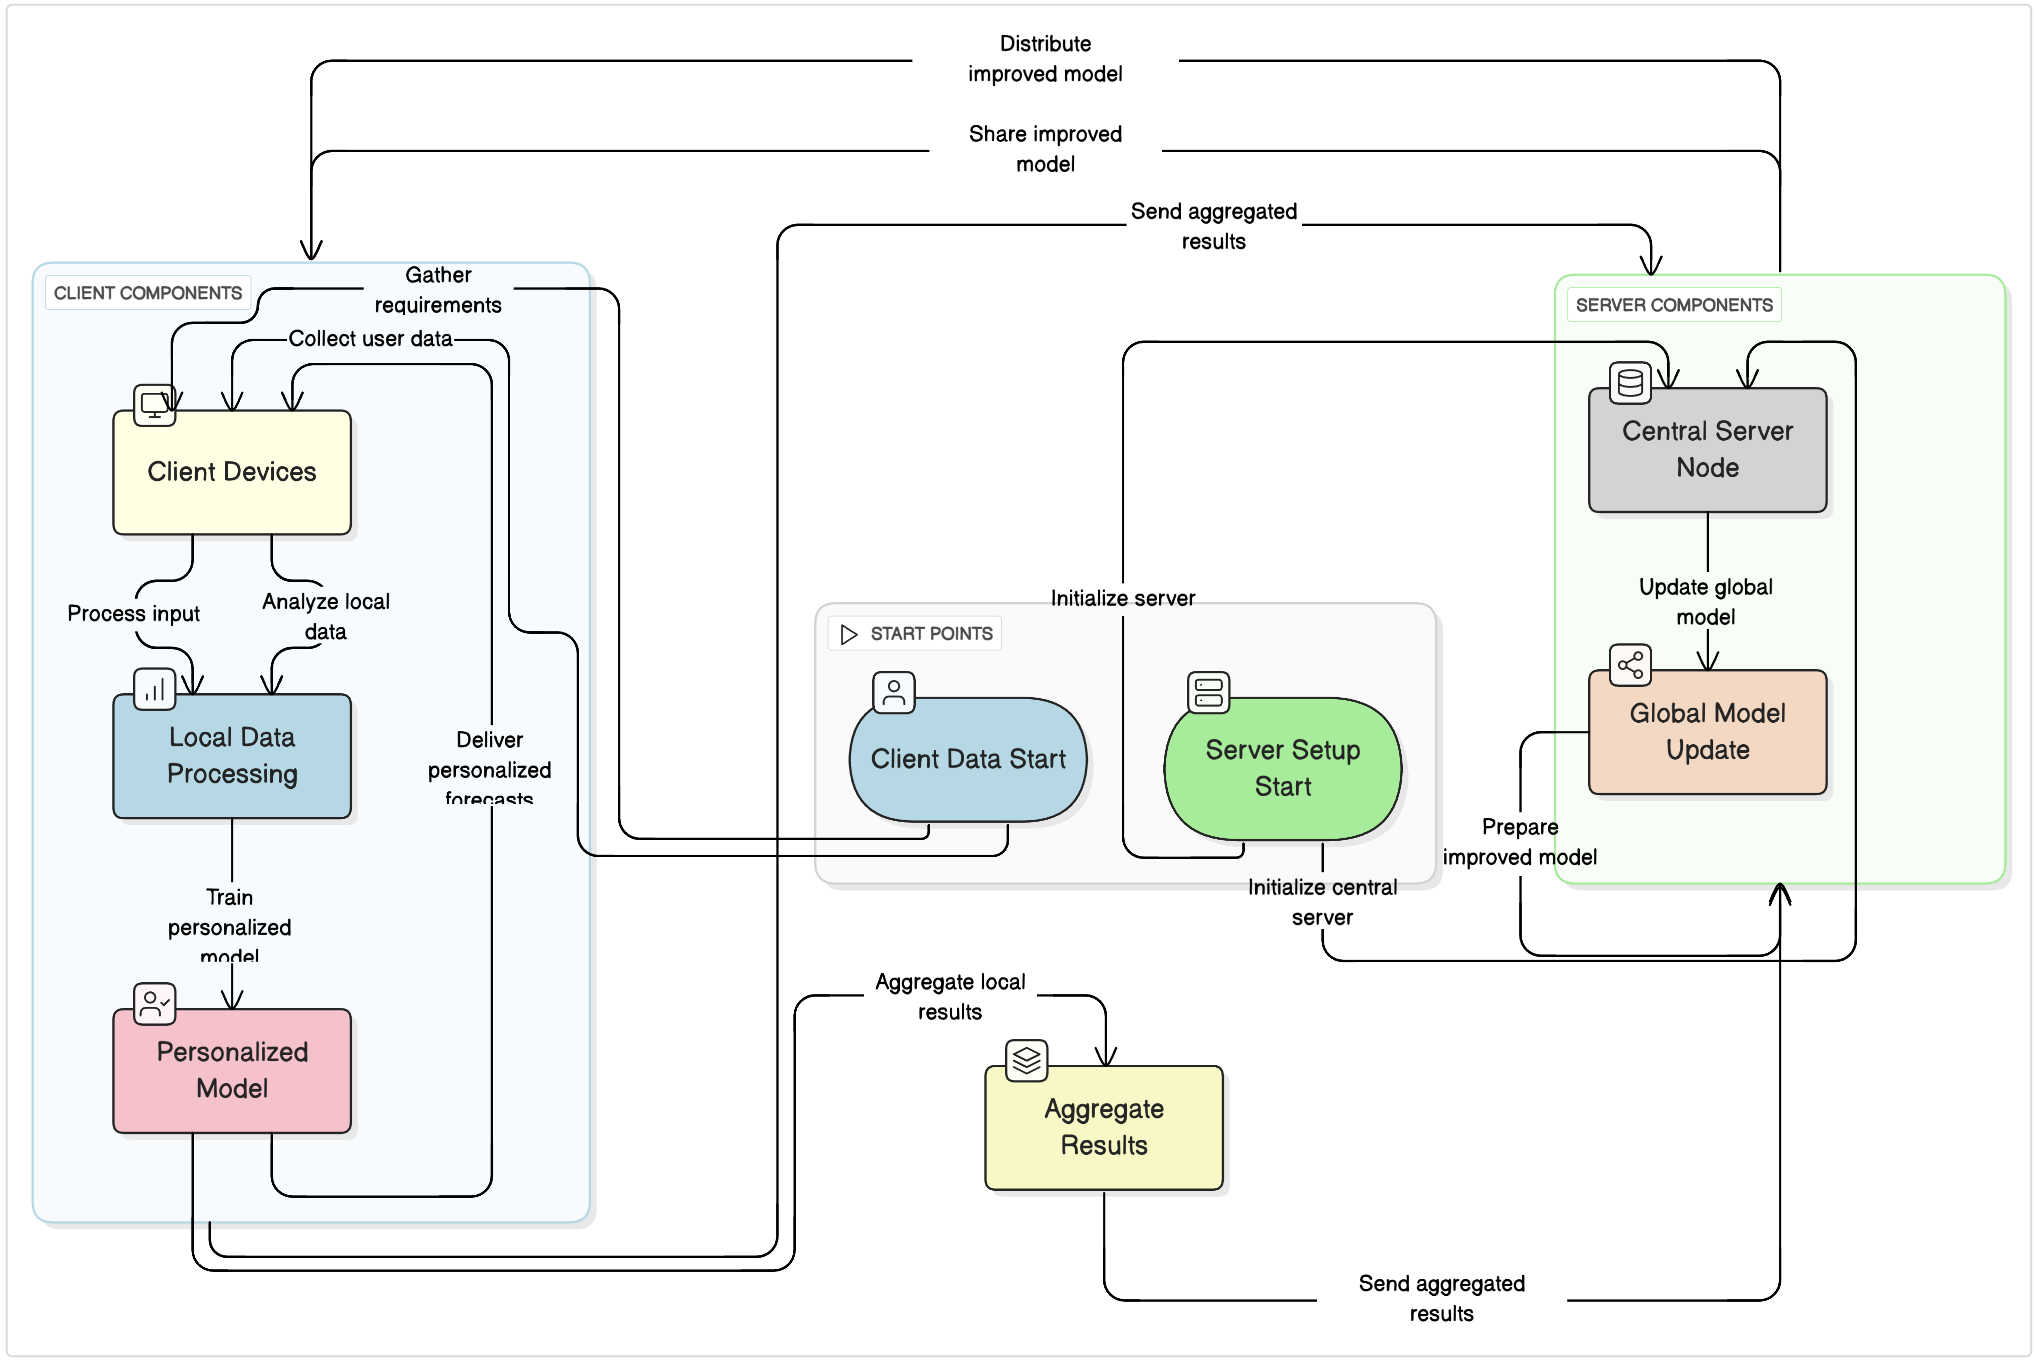
\includegraphics[width=0.9\linewidth, height=0.85\textheight, keepaspectratio]{SA_1.png}
\end{frame}

% --- APPLICATION WORKFLOW ---
\begin{frame}{Workflow}
    \framesubtitle{End-to-End Process Flow}

    \begin{columns}
        \begin{column}{0.5\textwidth}
             \begin{enumerate}
                \item \textbf{Data Collection:} Client collects time-series data locally
                \vspace{0.2cm}
                \item \textbf{Local Analytics:} Extract trends, anomalies, and insights
                \vspace{0.2cm}
                \item \textbf{Model Training:} Personalized forecasting model trained locally
                \vspace{0.2cm}
                \item \textbf{Secure Sharing:} Only model updates \& insights sent to server
                \vspace{0.2cm}
                \item \textbf{Global Aggregation:} Server aggregates updates into global model
                \vspace{0.2cm}
                \item \textbf{Distribution:} Improved global model sent back to all clients
            \end{enumerate}
        \end{column}
        
        \begin{column}{0.5\textwidth}
            \centering
            % Aligned and scaled to fit column
            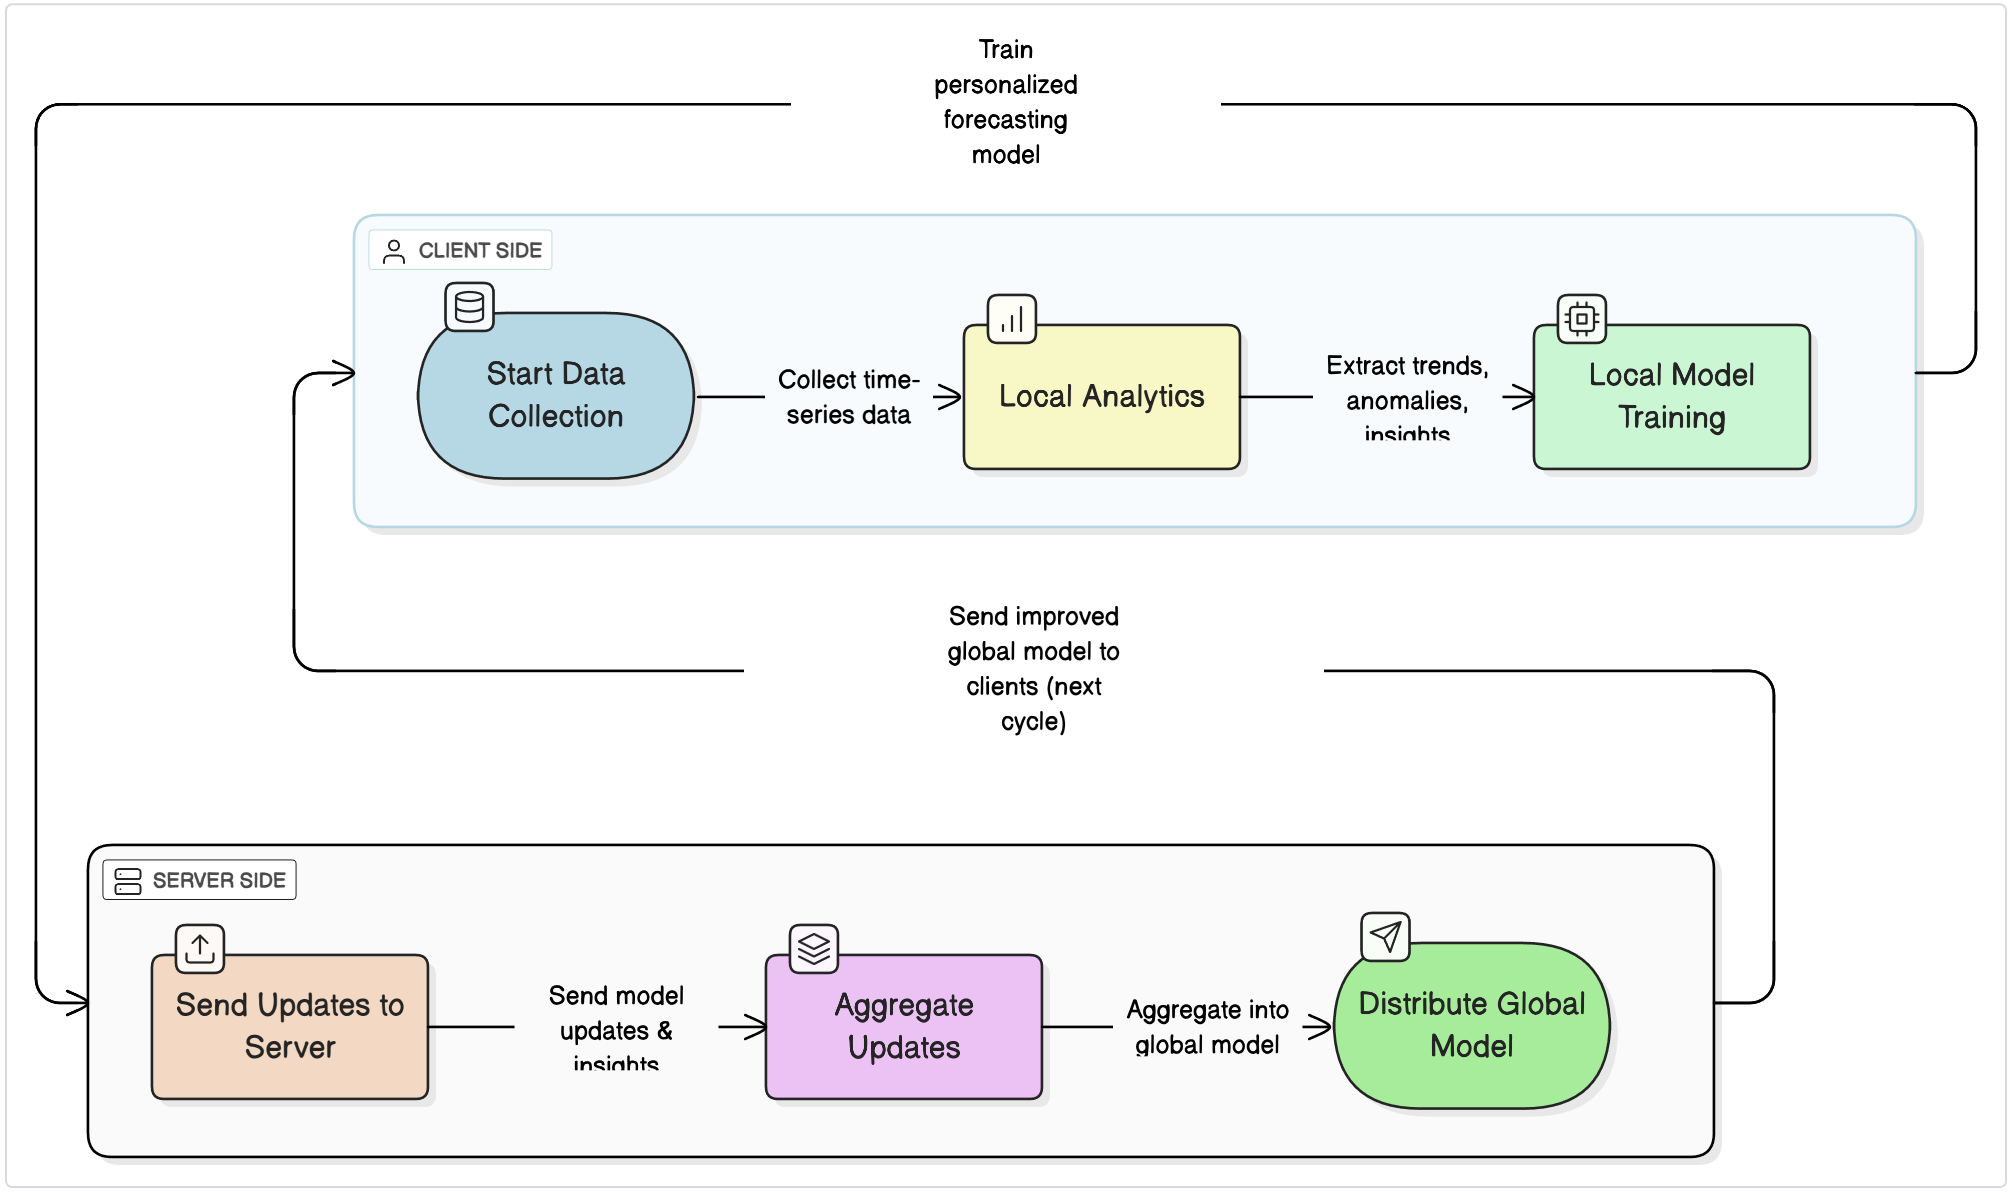
\includegraphics[width=1\linewidth, height=0.75\textheight, keepaspectratio]{AWF.PNG}
        \end{column}
    \end{columns}
\end{frame}

% --- DATA FLOW ---
\begin{frame}{Data Flow / Communication}
    \framesubtitle{Privacy-Preserving Architecture}

    \textbf{Key Principles:}
    \begin{itemize}
        \item Raw data stays on client devices
        \item Local analytics $\rightarrow$ model updates $\rightarrow$ server
        \item Server aggregates updates securely
        \item No raw data transmission
        \item Validation and aggregation ensure privacy
    \end{itemize}

    \vspace{0.5cm}
    \centering
    \textbf{Data Flow:} \\
    Input $\rightarrow$ Local Processing $\rightarrow$ Model Update $\rightarrow$ Global Aggregation $\rightarrow$ Output
\end{frame}

% --- TOOLS & TECHNOLOGIES ---
\begin{frame}{Tools, Technologies \& Protocols}
    \framesubtitle{Technical Stack}

    \begin{columns}
        \begin{column}{0.5\textwidth}
            \textbf{Frontend:}
            \begin{itemize}
                \item Web-based dashboard
                \item HTML, CSS, JavaScript
            \end{itemize}

            \vspace{0.3cm}
            \textbf{Backend:}
            \begin{itemize}
                \item Python (FL logic)
                \item REST API
            \end{itemize}

            \vspace{0.3cm}
            \textbf{Models:}
            \begin{itemize}
                \item LSTM / Transformer
                \item Time-series forecasting
            \end{itemize}
        \end{column}

        \begin{column}{0.5\textwidth}
            \textbf{Libraries:}
            \begin{itemize}
                \item TensorFlow / PyTorch
                \item NumPy, Pandas
            \end{itemize}

            \vspace{0.3cm}
            \textbf{Protocols:}
            \begin{itemize}
                \item REST API
                \item HTTP/HTTPS
            \end{itemize}

            \vspace{0.3cm}
            \textbf{Security:}
            \begin{itemize}
                \item Encrypted communication
                \item No raw data transmission
            \end{itemize}
        \end{column}
    \end{columns}
\end{frame}



% --- TECHNICAL ADVANTAGES ---
\begin{frame}{Technical Advantages of Proposed Framework}
    \framesubtitle{Research-Level Contributions}

    \small
    \begin{columns}
        \begin{column}{0.5\textwidth}

            \begin{block}{Privacy-Preserving Optimization}
                Federated gradient aggregation ensures raw multivariate time-series data remains local while only encrypted model parameters are shared.
            \end{block}

            \vspace{0.2cm}
            \begin{block}{Heterogeneity-Aware Personalization}
                Hybrid global backbone with client-specific layers handles non-IID distributions and improves localized forecasting accuracy.
            \end{block}

            \vspace{0.2cm}
            \begin{block}{Drift-Adaptive Learning}
                Integrated CUSUM-based concept drift detection enables automatic retraining under non-stationary temporal dynamics.
            \end{block}

        \end{column}

        \begin{column}{0.5\textwidth}

            \begin{block}{Attention-Based Explainability}
                Temporal attention mechanism computes timestep importance weights for interpretable multivariate forecasting.
            \end{block}

            \vspace{0.2cm}
            \begin{block}{Communication-Efficient Scalability}
                Weighted federated aggregation minimizes communication overhead while supporting multi-client deployment.
            \end{block}

            \vspace{0.2cm}
            \begin{block}{Unified Integrated Pipeline}
                Single framework jointly integrates FL, personalization, drift monitoring, and XAI — eliminating isolated module design.
            \end{block}

        \end{column}
    \end{columns}
\end{frame}
% % --- ADVANTAGES ---
% \begin{frame}{Advantages of Proposed System}
%     \framesubtitle{Key Benefits}

%     \begin{columns}
%         \begin{column}{0.5\textwidth}
%             \begin{block}{Privacy}
%                 \textbf{Strong privacy preservation}\\
%                 Raw data never leaves devices
%             \end{block}

%             \vspace{0.3cm}
%             \begin{block}{Personalization}
%                 \textbf{Personalized predictions}\\
%                 Per-client model adaptation
%             \end{block}

%             \vspace{0.3cm}
%             \begin{block}{Explainability}
%                 \textbf{Explainable insights}\\
%                 Supporting decision-making
%             \end{block}
%         \end{column}

%         \begin{column}{0.5\textwidth}
%             \begin{block}{Scalability}
%                 \textbf{Scalable architecture}\\
%                 Multiple organizations
%             \end{block}

%             \vspace{0.3cm}
%             \begin{block}{Adaptability}
%                 \textbf{Adaptive to changes}\\
%                 Drift detection and handling
%             \end{block}
%         \end{column}
%     \end{columns}
% \end{frame}

% --- REFERENCES ---
\section{References}
\begin{frame}[allowframebreaks]{References}
    \tiny
    % Citations to trigger bibliography generation
    \nocite{churaev2023,jothimurugesan2022,arivazhagan2020,mcmahan2017,liu2022}
    \nocite{yang2025mvfl,kalakoti2025fedxai,noseda2025financial,karamanlioglu2025clinical,wang2025personalized}
    \nocite{abdelsater2024llama,maher2025automl,gupta2025privacy,yuan2024trend,tang2025horizon}
    \nocite{zhang2022multitask,larocca2021attention,amato2023clustering,larocca2022shap,bernardi2023adaptive}
    \nocite{dusing2025sepsis,qayyum2023fedsepsis,lei2025supervised,pan2025multiprog,maurya2025secure}

    \bibliographystyle{IEEEtran}
    \bibliography{ref}
\end{frame}

% --- THANK YOU ---
\begin{frame}
    \centering
    {\Huge \textbf{\textcolor{amritaMaroon}{Thank You}}}

    \vspace{1cm}
    {\large Questions?}
\end{frame}

\end{document}